\documentclass{article}
\usepackage{graphicx}
\usepackage{hyperref}

\begin{document}

\title{The HypeDyn 2 Hypertext Fiction Editor\\Tutorial 4: Number Facts}
% \author{Alex Mitchell}
\date{}

\onecolumn
\maketitle

\tableofcontents

\section{Introduction}
In this tutorial, we will introduce ``number facts'', which are similar to text facts and true\slash false facts but can be used to store \textit{numbers}. Number facts can be updated to a specific number, to the value stored in another number fact, or to a random number. You can also perform simple math on number facts, and use number facts in conditions. We will be creating a variation of the ``Little Red Riding Hood'' hypertext fiction which you created in tutorial 1. We will change the story such that the choice of ending is determined by a number fact, which can either be preset by the author or chosen randomly when the story is being read. We will also change the side path (``Hood details'')
such that it is unlocked, not after the first reading, but instead after the \textit{second} reading, through the use of a counter.

% number facts:
% create number fact
% update number fact using: input, fact, math, random
% update text using: number fact
% conditions: 
% - examples of order of execution, using stop-if-true, intermediate fact for
% complex calculation, several rules working together in one link/node rule
% - explain about what is triggered when (in sidebar?)
% random? - random endings: woodsman may or may not show up to save Red

The nodes and facts in the final story are shown in Figure
\ref{fig:tut3:completed}.

\begin{figure}[h]
  \centering
  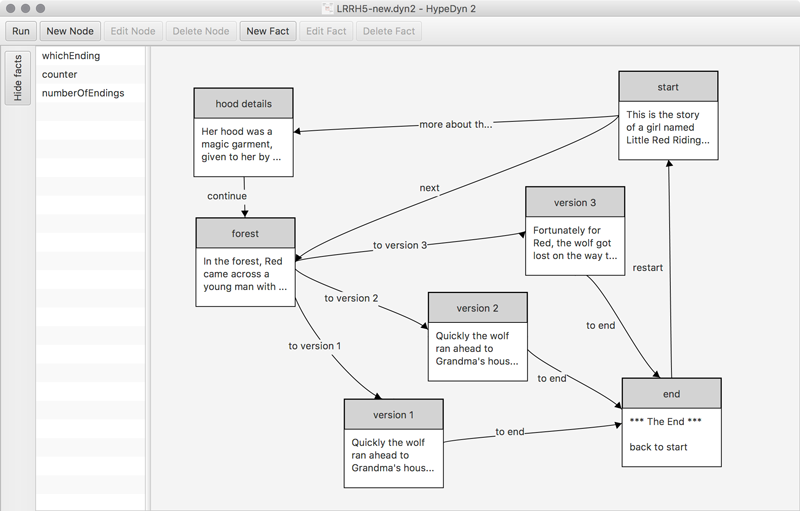
\includegraphics[width=12cm]{images/hypedyn-tutorial-4-figure-1}
  \caption{\textit{The completed ``Little Red Riding Hood'' story.}}
  \label{fig:tut3:completed}
\end{figure} 

\textit{Note:  HypeDyn is a work-in-progress. If you encounter any errors, please report them as issues on our Github site: \url{https://github.com/narrativeandplay/hypedyn2}.}

\section{Getting started}

First, open HypeDyn 2 by double-clicking on the file \textbf{HypeDyn2.exe} (in Windows) or \textbf{HypeDyn 2.app} (in MacOS).

We will continue from the story that you created in tutorial 1. If you don't have the story, you can start from the file \textsc{LRRH.dyn2} in the \textsc{examples} folder. HypeDyn 2 files always end with a \textbf{.dyn2} extension. Once you've opened \textsc{LRRH.dyn2}, save the file under a different name, such as \textsc{LRRH5.dyn2}.

\section{Creating a number fact}

Number facts are similar to the text facts and true/false facts which 
were introduced in Tutorial 3. Instead of keeping track of text or 
boolean values, number facts are \textit{integers}, meaning they can be set  to any positive or negative ``natural'' or ``whole'' number ie. \dots -3, -2, -1, 0, 1, 2, 3 \dots, but not \textit{real} numbers with a 
decimal place. Number facts can be tested in conditions, and set in 
actions.

The first feature we will introduce is the use of a number fact in a condition. As with other conditions, this allows you to determine which actions should be triggered, either when a node is entered or when a fragment is clicked.

\subsection{Creating the fact}
% - create a number fact: whichEnding?

We will begin by creating the number fact.

\begin{enumerate}
  \item In the main HypeDyn window, click on the \textit{New Fact} button.
  \item In the \textit{New Fact} window, set the \textit{Fact Type} to ``Number fact''.
  \item Name the fact ``whichEnding?''.
  \item Leave the \textit{Initial value} as ``0'', and click "Ok". As with other  facts, your new fact will appear in the fact list on the  left side of the main window.  
\end{enumerate}

We now have a \textit{number fact} which we can use to keep track of 
numeric values. Eventually we will use this fact to store a random number that we will use to choose the ending. Before we do this, we will first introduce how to set a number fact, and then use the value of the number fact to go to different endings.

\subsection{Creating the alternative endings}
% - make two endings: version 1 and version 2

What we want to do with our ``whichEnding?'' number fact is use it to 
determine which of two possible endings will be visited when the 
reader clicks on ``next'' in the ``forest'' node. Currently it leads 
to the node ``end''. We will now create 2 new nodes, ``Version 1'' 
and ``Version 2'', which will be shown depending on the value of 
``whichEnding?''. Create two nodes:

% should continue the numbering here, do this later
\begin{enumerate}
  \item \textit{Name}: Version 1\\
  \textit{Content}: 
  \begin{quotation}
  \noindent Quickly the wolf ran ahead to Grandma's house, swallowed 
  Grandma whole, and disguised himself as the poor old lady. When Red 
  arrived, he finished her off too. Yum! \\

  \noindent next
  \end{quotation}
  \item \textit{Name}: Version 2\\
  \textit{Content}: 
  \begin{quotation}
  \noindent Quickly the wolf ran ahead to Grandma's house. 
  Unfortunately for the wolf, Grandma's friend the Woodcutter had 
  stopped by for tea, and he finished the wolf off with one swipe of 
  his axe. Poor wolf! \\

  \noindent next
  \end{quotation}
  \item Add a link from the ``next'' text in each node to the ``end'' node.
\end{enumerate}


\subsection{Setting the number fact}
% - set number fact in node rule for ``forest''

We want to have the reader go from the ``next'' link to ``Version 1'' 
if ``whichEnding?'' is equal to 1, and to ``Version 2'' if 
``whichEnding?'' is equal to 2. Before we can do this, however, we 
need to set the value of ``whichEnding?'' As with other types of 
facts, a number fact can be updated in either a node rule or a fragment 
rule. We will use the node rule in the ``forest'' node to set the 
value.      

\begin{enumerate}
    \item Edit the ``forest'' node, and select the \textit{Node rules} tab.
    \item Add a node rule, and name the rule ``choose ending''.
    \item Add an ``Update number fact'' action.
    \item In the new action, choose fact ``whichEnding?'' for the fact.
    \item Notice that there are several options in the ``using'' pulldown menu. Number facts can be updated based on a number that the author inputs directly (the \textit{Input} option), much like specifying Input when updating text on a fragment. They can also be updated using another fact, using a mathematical expression, or using a random number.
    
For now, we want to specify the number directly, so choose ``Input''. In the input field, specify ``1''.
\end{enumerate}

\noindent The rule we've created will set the ``whichEnding?'' fact to 1 when the reader enters the ``forest'' node.

\subsection{Displaying a number fact using conditional text}

To check whether our new rule is working, we can temporarily add a fragment which we will use to display the current value of ``whichEnding?'' This technique is a useful way to debug your stories when using number facts.

\begin{enumerate}
    \item At the end of the ``forest'' node, add the text ``whichEnding? =  dummy''. We will replace the text ``dummy'' with the current value of whichEnding?
    \item Create a fragment on the text ``dummy'', name the fragment ``debugging'', and edit the fragment's rules.
    \item Add a rule to the fragment, and name the rule ``debugging''.
    \item Add an ``Update fragment text'' action to the rule, and choose to update text using ``number fact''. In the pulldown menu, choose the fact ``whichEnding?''
    \item Now run the story. Notice that the text ``dummy'' is replaced with the value ``1''.
    \item Edit the ``forest'' node's node rules, go into the ``choose ending'' rule, and change the ``update fact using'' action so that the value is 2. 
    \item Run the story again. You should see that the value displayed in the forest node is now ``2''.
\end{enumerate}

\noindent Now that we've created our number fact, and have set it to a specific value, we can use this number fact to decide which ending to show.

\section{Comparing number facts}

% - now make use of this in a condition
We will now add a condition to the ``to the end'' fragment rule in the ``forest'' node that checks the value of the ``whichEnding?'' fact. 
If the value is 1, the link will go to ``Version 1'', and if the 
value is 2, the link will go to ``Version 2''.

\subsection{Adding the first rule}

We'll begin by adding the rule which takes us to ``Version 1''.

\begin{enumerate}
    \item Edit the ``forest'' node, and then edit the ``to the end''  fragment's rules. You should see the ``to the end'' rule which we created in tutorial 1.
    \item Edit the ``to the end'' rule. It currently contains one action, ``follow link to end''. Rename the rule ``to version 1''.
    \item Now change the action to ``follow link to Version 1''. This is the action we will use if ``whichEnding?'' is 1.
    \item Add a condition. Choose ``Number Fact'' as the type of condition in the first pulldown menu.
    \item Notice that after changing the condition to a number fact 
    condition, the condition changes to show three pulldown menus. The first pulldown menu contains a list of number facts. Choose the ``whichEnding?'' fact.
    \item The second pulldown menu contains \textit{$<$}, \textit{$>$}, \textit{$\le$}, \textit{$\ge$}, \textit{=} and \textit{not =}. This is the \textit{comparator} which will be used to compare the chosen number fact (in this case ``whichEnding?'') with the right-hand side of the condition.
    
For now, set the comparator to be ``=''.
    \item To the right of the comparator is another pulldown menu, which has two options: input and fact. Choosing ``Input'' lets you enter a specific number for the comparison, whereas choosing ``Fact'' lets you compare against another fact. Set the choice to ``Input''.
    \item In the text entry field, enter ``1''. This means that the actions listed in the rule will be triggered when ``whichEnding?'' is equal to 1.
\end{enumerate}

\subsection{Testing the first rule}

At this point, we've created the rule which will take the reader to node ``Version 1'' if the fact ``whichEnding?'' is equal to 1. Recall that we have currently set the node rule in the ``forest'' node to set ``whichEnding?'' to 2. What will happen if we run the story now?

\begin{enumerate}
    \item Run the story.
    \item Notice that the link on the text ``next'' in ``forest'' is disabled -- this is because it contains rule with a ``follow link to'' action, but that rule's conditions are not satisfied.
    \item Now edit the ``choose ending'' node rule in the ``forest'' node, and change the ``update fact'' action so that ``whichEnding?'' is set to 1.
    \item Run the story again. This time, the link is enabled. Click on the link, and you will be taken to node ``Version 1''.
\end{enumerate}

\subsection{Adding the second rule}

% - create condition that checks if 1 or 2 (stop if true used)

Now we need to add the second rule, which will take the reader to 
node ``Version 2'' if ``whichEnding?'' is 2.

\begin{enumerate}
    \item Edit the ``to the end'' fragment's rules in the ``forest'' node.
    \item We are going to add a second rule, which should only ever be triggered if the first rule, ``to version 1'', was \textbf{not} satisfied. To make sure that HypeDyn stops checking rules after a given rule is satisfied, you can check the ``Stop if true'' option on a rule. Do this now on the rule ``to version 1''.
    \item Add a rule, and name the rule ``to version 2''.
    \item Add an action ``follow link to Version 2''.
    \item We only want this rule to be triggered if ``whichEnding?'' is set to 2, so we need to add a condition to check this. 

    % stop if true discussion - why put the stop if true if we're 
    % also putting a condition? for efficiency
    
Add a condition to the rule, and set it to ``Number fact whichEnding? = input 2''.
    \item Run the story. When you get to ``forest'' and click on the ``next'' link, you should go to ``Version 1''.
    \item Now edit the node rule for ``forest'', and change the ``choose ending'' rule so that ``whichEnding?'' is set to 2.
    \item Run the story again. This time, the ``next'' link should take you to ``Version 2''.
\end{enumerate}

\noindent We have now successfully created a fragment which links to different destinations based on a number fact.

%One thing to note is that both the ``Stop if true'' option on the 
%``to version 1'' rule and the condition in the ``to version 2'' rule 
%will ensure that the second rule is only triggered if 

% Note: not sure how useful this next bit is
% - could use a fact rather than typing in the number
% - create fact preferredEnding
% - set to 1 in start node, then set whichEnding to fact preferredEnding

\section{Using random numbers}

% - but this isn't very interesting - why not make it random?
Although we've created a set of rules which use number facts to determine which node to visit next, this isn't really anything which we couldn't have done with, for example, a true\slash false fact. One way to make this more interesting, and to show what can be done with number facts, is to set the fact ``whichEnding?'' to a \textit{random number}. 

\subsection{Setting the random number in a node rule}

We will now create a rule which sets ``whichEnding?'' to a random number. There are several places where we could put this rule. To start with, we will change the ``choose ending'' node rule in the ``forest'' node to update ``whichEnding?'' to a random number, rather than a number which we decided when writing the story.

% edit node rule, instead of setting to fact, set to random between input 1
% and input 2
\begin{enumerate}
    \item Edit the ``choose ending'' rule in the node rules for the  ``forest'' node.
    \item There is currently one action: ``update fact Number  whichEnding? using Input 2''. Change the ``using'' pulldown to  ``random''. Notice that there are now two pulldown menus to the right of ``random''. These input fields allow you to choose the lower and upper range of the random number that will used to update the number fact. These bounds can be specified either using Input or a Fact. For now, set both pulldown menus to Input. An input field will be created beside each pulldown menu.
    \item We want a random number between 1 and 2, since there are 2 versions of the ending. So enter ``1'' in the first input field, and ``2'' in the second input field. 
    \item Click ``Ok'' to close the Edit Node window. Now run the story. When you enter the ``forest'' node, the value displayed at the bottom of the node should be either 1 or 2.
    \item To convince yourself that the value is being chosen randomly, click on the ``back'' button, and then click on the ``forest'' link again. Do this a few times. Notice that sometimes the same number appears two or more times in a row -- this is because the number is chosen randomly, without regard to what the previous value was. 
    % aside: if you wanted it to alternate, how would you do this?
\end{enumerate}

\subsection{Setting the random number in a fragment rule}

% or could do it when the link is clicked - useful to show order of 
% evaluation
Note that although we put the update fact action which sets ``whichEnding?'' on the node rule for the ``forest'' node, instead we could have put the action on the ``next'' fragment itself. One advantage of having the action on the node rule is we can see the value of the ``whichEnding?'' fact (on the ``dummy'' fragment in the node's text), which helps with debugging. However, it can sometimes be useful to put actions such as this on a fragment. To show how this is done, we will now put the same action that we put in the node rule into a fragment rule on  the ``next'' fragment.

\begin{enumerate}
    \item Edit the ``next'' fragment's rules in the ``forest'' node.
    \item There are already two rules on the fragment: ``to version 1'' and ``to version 2''. We want to update the ``whichEnding?'' fact, and \textit{then} check the value of the fact. Remember that HypeDyn checks, and then triggers, rules in the order they are listed in the rules list. This means that we will have to put our new rule \textit{before} the two existing rules.
    
Add a new rule. Notice that it appears at the end of the list of fragment rules. We need to move it up so that it is before ``to version 1''.
    \item Click on the ``up'' button to the left of your new rule. The rule should have moved up, so that it is now before ``to version 2'', but still after ``to version 1''.
    \item Click ``up'' again. The new rule should now be first in the list, before ``to version 1''.
    \item Name the new rule ``randomize''.
    \item Add an ``Update number fact'' action, and set it to ``update number fact Random Input 1 Input 2''.
    \item Try running the story, and clicking the ``next'' link several times. Notice that the destination the link goes to is not always the same as what you would expect based on the number displayed in the ``forest'' node. This is because the ``next'' link's first action is again randomizing the value in ``whichEnding?''
\end{enumerate}

\subsection{Adding a third ending}

% - what if we add a third ending? need to change both randomizations
% - instead, make a ``numberOfEndings'' fact, set in start node, use this
% instead (replace above update from fact with this?)

Note that it is not very good form to have two different places where 
``whichEnding?'' is randomized, as you may lose track of where the 
randomization is taking place. There is also another problem -- if we 
add another ending, we now need to remember to change the upper bound 
for the random number from two to three in two different places!

Sometimes there are good reasons for having randomization such as 
this happening in several places. For example, there may be several 
different nodes which lead to the endings, each of which need to do 
some randomization based on the number of endings. One way to improve 
the situation is to use a \textit{fact} for the upper bound, rather 
than a number we have typed in two different places. Then we can just 
change the value of the fact, and everywhere the fact is used, we'll 
get the correct value. We will do that now.

\begin{enumerate}
    \item First, we'll make a third version of the ending. Create a new node, and name it ``Version 3''.
    \item Enter the following text in the node:
    
    \begin{quotation}
    \noindent Fortunately for Red, the wolf got lost on the way to Grandma's house.\\

    \noindent next
    \end{quotation}
    \item Add a link from the text ``next'' to the ``end'' node.
    \item Now we will add a new number fact to keep track of how many endings there are. Create a new number fact, and name it  ``numberOfEndings''.
    \item We need this fact to be set to ``3''. To do this, you can set the \textit{Initial value} of the fact in the \textit{New fact} dialog to be 3. 
    
Note that if you want to change this value later, you can select the fact in the \textit{Fact list} and click on the \textit{Edit Fact} button, or double-click the fact in the \textit{Fact list}.
    \item Now we need to make use of this new fact in our two rules where we randomize ``whichEnding?''.
    
Edit the ``forest'' node, and edit its node rules. Edit the rule ``choose ending''. In the first action, change the second ``Input'' to ``Fact''. This is the upper bound of our random number. Choose the fact ``numberOfEndings''.
    \item Now do the same for the ``randomize'' rule in the ``to the end'' fragment's rules.
    \item Finally, we need to add a rule to the ``to the end'' fragment to take the reader to node ``Version 3'' if ``whichEnding?'' is equal to 3.
    
Add a rule to the ``to the end'' fragment's rules, and name it ``to version 3''. Make sure the rule is at the end of the list of fragment rules.
    \item Add the condition ``Number Fact whichEnding? = Input 3''.
    \item Add the action ``follow link to Version 3''.
\end{enumerate}

\noindent Now try running the story. You should be able to follow the ``next'' link in the ``forest'' node, and have it randomly take you to one of the three endings.

In this section, we introduced the use of a random number fact to create a fragment which randomly links the reader to different destinations. This is a powerful procedural technique. It can, however, be problematic if misused. If choices the reader is making result in random outcomes, the reader may begin to doubt that her choices have any real impact on the story. This may or may not be what you intend as an author.

\section{Using a counter}

% - counter: unlock side path on third reading
In this section, we will introduce another way in which authors can 
use number facts to make their stories more procedural. Here, we will 
update facts based on math. We will demonstrate this by implementing 
a \textit{counter} which unlocks a side path in the story after the 
reader has reread the story a certain number of times. To do this, we 
will create a new number fact, named ``counter''. Each time the 
reader clicks on the ``restart'' link from the ``end'' node back to 
the ``start'' node, we will add 1 to ``counter''. Then, in the ``more 
about the hood'' link, instead of checking whether or not the ``end'' 
node has been visited, we will check the value of ``counter'', and 
enable the link when the target value has been reached.

\subsection{Creating the counter}

First we will create a number fact to act as our counter.

% - add ``counter'' number fact
\begin{enumerate}
    \item Create a new number fact, and name it ``counter''. We'll 
    use this to keep track of the number of times the reader has gone 
    back to the start of the story from the ``end'' node.
    \item So that we can see how the counter is changing, we will use 
    a technique similar to what we did with the ``whichEnding?'' fact 
    to display the value of ``counter''.
    
    Edit the ``end'' node, and add the text ``counter=placeholder'' 
    between the text ``*** The End ***'' and the link ``back to 
    start''. Add a fragment on the text ``placeholder'', name the fragment 
    ``show counter'', and add a rule which has the action ``update 
    text using number fact counter''. This will show us the value of 
    ``counter'' when we test our story.
\item Now run the story. When you get to the ``end'' node, notice that the 
value shown for ``counter'' is ``0''. 
\end{enumerate}

\noindent Note that facts are always automatically updated to the value you set for their \textit{Initial value} when the story is started. In this case, we set the initial value to be 0, which is exactly what we want. 

\subsection{Incrementing the counter}

When the reader goes back to the start the first time, we will add 1 to the current value of counter, updating counter to 1.

% - add ``update number fact counter using math fact counter + input 1'' to
% ``restart'' link in ``end''
\begin{enumerate}
    \item Edit the ``restart'' fragment in the ``end'' node. 
    \item There is already one rule, ``restart'', which was added in 
    Tutorial 1. This rule contains one action, ``follow link to 
    start'', which takes the reader back to the ``start'' node. In 
    addition, we want to increment the counter fact when the reader 
    goes back to the ``start'' node.
    
    Add an ``Update number fact'' action to the ``restart'' rule. Select Fact ``counter'', and set the ``using'' pulldown menu to ``Math''.
    \item After you choose ``Math'' for the ``using'' pulldown menu, you will see three pulldown menus: one to set the first value of the expression, the second to set the operator, and the third to set the second value. These menus let you specify the \textit{math expression} which will be triggered for this action. 
    
HypeDyn lets you update number facts using simple math expressions. Each one consists of two values (either an Input or a Fact), and an \textit{operator}: +, -, x, / (div) and \% (mod). Because number facts are whole numbers, the ``/'' operator is actually ``div'', which performs the division but discards the remainder. The ``\%'' operator is called ``mod'', which performs the division and gives you the remainder.
    
We want to add 1 to the current value of ``counter''. To do this, choose ``Fact'' for the first value. You will see a new pulldown menu containing a list of number facts. Choose ``counter''.
    \item For the second value, we want to add 1, so set the second value's pulldown menu to ``Input'', and enter ``1'' into the text field that appears after the pulldown menu. 
    \item Finally, we want to perform addition on the two values, so set the operator pulldown to ``+''.
\end{enumerate}

Try running the story now. Click through to the ``end'' node, and then read the story a second time by following the ``back to start'' link. When you reach the ``end'' node a second time, you should see the text ``counter=1''. Try rereading several times, and you'll see the counter increase by 1 each time.

\subsection{Using the counter to unlock the side path}

% - change condition on ``more about the hood'' to ``number fact counter = input
% 2''
We can now make use of this counter to unlock the ``more about the hood'' side path after the reader has gone through the story twice, rather than just once.

\begin{enumerate}
    \item Edit the ``more about the hood'' fragment in the ``start'' node, and edit the ``more about the hood'' rule. This rule was added in Tutorial 1. It contains one condition, ``Node end visited'', and one action, ``follow link to Hood Details''. 
    \item We want to retain the existing action, but instead of triggering the rule if the ``end'' node has been visited, we want to trigger it only if the ``end'' node has been visited \textit{two times}.To do this, we will use our ``counter'' fact, and use a number fact condition to check the value of the fact. 
    
Change the type of the condition to ``Number Fact'', and choose fact ``counter''.
    \item We want to check whether the reader has visited the ``end'' node at least twice, so set the comparator pulldown menu to show ``='', and make sure the type pulldown menu for the right-hand side is set to ``Input''. Then type the value ``2'' in the text entry field.
\end{enumerate}

% - run - what if read 3 times?
% - instead try $\ge$ input 2
\noindent Now try running the story. Read through once, and then go back to the ``start'' node by clicking on the ``back to start'' link in the ``end'' node. Notice that the link on the text ``red hood'' is not clickable. Now continue to read, and once again to back to the start. This time, the second time you've gone back to the start, the ``red hood'' link \textit{is} clickable.

What do you think will happen if you read through again, and then go 
back to the start a \textit{third} time? Try it. Why isn't the link clickable the third time?

Remember, we set the condition on the fragment to be ``Number fact counter = 2''. This means that the link is clickable when ``counter'' is \textit{exactly} equal to 2. This is fine if we want the link to only be available on the second rereading. If, however, we want it to be unlocked for every subsequent rereading, we should use ``$\ge$'' instead of ``=''. Try this, and then read the story again. This time, you should see the ``red hood'' link is clickable for the second and subsequent rereadings.

% leave this as an exercise in ``next steps'' below :)
% make it so that it doesn't let you re-read more than 3 times
% - show problem with putting 2 separate rules on ``restart'' link (LRRH5d.dyn
% and LRRH5e.dyn)
%There is one last thing that we'll do. Since we have a counter, it is 
%possible to \textit{limit} the number of times that the reader can 
%reread the story. We will now limit the number of rereadings to 3, by 
%settting the ``back to start'' link in the ``end'' node to only be 
%clickable if counter $<$ 3, ie. if we have already reread (followed the 
%``back to start'' node) less than three times.

% maybe (later?) do something about procedural conversations? to show
% complexity?

\section{Next steps}

We have modified the original story from Tutorial 1, \textsc{LRRH.dyn2}, by adding random selection of endings, and by adding a counter which both unlocks the side path on the second rereading. The completed version of this story can be found in the file \textsc{LRRH5.dyn2}. 

There are several things that you could try to enhance the story. For  example, you limit the number of rereadings to three, making sure that once 
you prevent the reader from rereading you let them know why. You could also make sure that the reader doesn't get the same random ending twice in a row. One way of adding these enhancements can be found in \textsc{LRRH6.dyn2}. 

\section{Conclusion}

In this tutorial, we have created a simple hypertext fiction which makes use of randomization and a counter to procedurally alter the story which the reader encounters. This provides the basis for much more procedural approaches to creating interactive stories. See what you can think of, and then try it!

\end{document}